\documentclass[10pt,compress]{beamer}
%\documentclass[handout,t]{beamer}
\usepackage[portuguese,brazilian]{babel}
%\usepackage{mathtools}
\usepackage{booktabs}
\usepackage{amsmath,amsthm,amsfonts,cite,color,enumerate,subfig}
\usepackage{mathrsfs}
\usepackage{enumitem}
\usepackage{nicefrac}
\usepackage{subfig}
\usepackage{algpseudocode}
\usepackage{framed}
\usepackage{cancel} % Use \usepackage[thicklines]{cancel} for thicker strokes
\definecolor{cancelgray}{gray}{0.5}
\renewcommand{\CancelColor}{\color{cancelgray}}

\newtheorem{theorem}{Theorem}
\newtheorem{example}{Example}
\newtheorem{corollary}{Corollary}
\newtheorem{definition}{Definition}
\newtheorem{algorithm}{Algorithm}
\newtheorem{lem}[theorem]{Lemma}

% NEW COMMANDS
\renewcommand{\mod}[1]{\  (\mathrm{mod} \ #1)}
\newcommand{\qi}{\boldsymbol{i}}
\newcommand{\qj}{\boldsymbol{j}}
\newcommand{\qk}{\boldsymbol{k}}
\newcommand{\qmu}{\boldsymbol{\mu}}
\newcommand{\qnu}{\boldsymbol{\nu}}
\newcommand{\qV}{\boldsymbol{V}}
\newcommand{\sen}{\mathrm{\, sen \,}}
\newcommand{\red}[1]{{\color{red}#1}}
\DeclareRobustCommand{\rchi}{{\mathpalette\irchi\relax}}
\newcommand{\irchi}[2]{\raisebox{\depth}{\Large $#1\chi$}} % inner command, used by \rchi

% ISOMORPHISM SYMBOL
\makeatletter
\newcommand*{\isomorphism}{%
	\mathrel{%
		\mathpalette\@isomorphism{}%
	}%
}
\newcommand*{\@isomorphism}[2]{%
	% Calculate the amount of moving \sim up as in \simeq
	\sbox0{$#1\simeq$}%
	\sbox2{$#1\sim$}%
	\dimen@=\ht0 %
	\advance\dimen@ by -\ht2 %
	%
	% Compose the two symbols
	\sbox0{%
		\lower1.9\dimen@\hbox{%
			$\m@th#1\relbar\isomorphism@joinrel\relbar$%
		}%
	}%
	\rlap{%
		\hbox to \wd0{%
			\hfill\raise\dimen@\hbox{$\m@th#1\sim$}\hfill
		}%
	}%
	\copy0 %
}
\newcommand*{\isomorphism@joinrel}{%
	\mathrel{%
		\mkern-3.4mu %
		\mkern-1mu %
		\nonscript\mkern1mu %
	}%
}
\makeatother

\usepackage[utf8]{inputenc}
%\usepackage[T1]{fontenc}
\usepackage{longtable}
\usepackage{booktabs}

%\usepackage{enumitem} % For custom spacing in lists environments
%\setlist{nolistsep}
\usepackage{subfig}
\usepackage{float}
\usepackage{url} % Permite exibição de sites de forma organizada
\usepackage{color}
\usepackage{epigraph}
\definecolor{darkred}{RGB}{110, 0, 0}
\definecolor{darkred2}{RGB}{80, 0, 0}
\definecolor{darkblue}{RGB}{0, 0, 75}
\definecolor{paleblue}{RGB}{37, 125, 194}
\definecolor{mygray}{gray}{0.6}

% NEW COMMANDS
%\renewcommand{\mod}[1]{\  (\mathrm{mod} \ #1)}
%\newcommand{\ord}[1]{\mathrm{ord}(#1)}
\newcommand{\qi}{\boldsymbol{i}}
\newcommand{\qj}{\boldsymbol{j}}
\newcommand{\qk}{\boldsymbol{k}}
\newcommand{\qmu}{\boldsymbol{\mu}}
\newcommand{\qnu}{\boldsymbol{\nu}}
\newcommand{\qV}{\boldsymbol{V}}
\newcommand{\sen}{\mathrm{\, sen \,}}
\newcommand{\red}[1]{{\color{red}#1}}
% Novos comandos para colorir. São necessários porque a coloração de links via hyperref atinge também o menu, não fica legal.
\newcommand{\colorlink}[1]{{\color{paleblue}#1}}
\newcommand{\colorcite}[1]{{\color{mygray}#1}}

\usepackage[font={scriptsize},labelfont={scriptsize,color=darkred2}]{caption}


% LISTINGS
\usepackage{listings}
\lstset{ %
backgroundcolor=\color{white},   % choose the background color; you must add \usepackage{color} or \usepackage{xcolor}
basicstyle=\footnotesize,        % the size of the fonts that are used for the code
breakatwhitespace=false,         % sets if automatic breaks should only happen at whitespace
breaklines=true,                 % sets automatic line breaking
captionpos=n,                    % sets the caption-position to bottom
commentstyle=\color{cyan},    % comment style
%   deletekeywords={...},            % if you want to delete keywords from the given language
escapeinside={\%*}{*)},          % if you want to add LaTeX within your code
extendedchars=true,              % lets you use non-ASCII characters; for 8-bits encodings only, does not work with UTF-8
frame=single,	                   % adds a frame around the code
keepspaces=true,                 % keeps spaces in text, useful for keeping indentation of code (possibly needs columns=flexible)
keywordstyle=\color{blue},       % keyword style
language=Python,                 % the language of the code
%   otherkeywords={*,...},           % if you want to add more keywords to the set
numbers=left,                    % where to put the line-numbers; possible values are (none, left, right)
%   numbersep=5pt,                   % how far the line-numbers are from the code
numberstyle=\color{black}, % the style that is used for the line-numbers
rulecolor=\color{black},         % if not set, the frame-color may be changed on line-breaks within not-black text (e.g. comments (green here))
%   showspaces=false,                % show spaces everywhere adding particular underscores; it overrides 'showstringspaces'
showstringspaces=false,          % underline spaces within strings only
%   showtabs=false,                  % show tabs within strings adding particular underscores
stepnumber=5,                    % the step between two line-numbers. If it's 1, each line will be numbered
stringstyle=\color{magenta},     % string literal style
tabsize=2,	                   % sets default tabsize to 2 spaces
%   caption=\lstname                   % show the filename of files included with \lstinputlisting; also try caption instead of title
}

%\usepackage{lipsum}
\usepackage[portuguese]{algorithm2e}

\usepackage{hyperref}
\hypersetup{
colorlinks=false,
% 	citecolor=darkred,
% 	linkcolor=.,
}
% Obs.: The command \texorpdfstring from the hyperref package allows for \textsubscript{} and math symbols in sectioning headings.

% Math packages
\usepackage{amsmath}
\usepackage{amsthm}
\usepackage{amsfonts}
\usepackage{amssymb}
\usepackage{mathrsfs}
\usepackage{nicefrac}
\usepackage{amsthm}
\usepackage{bm} % for nice bold symbols
\usepackage{upgreek} % for upright greek letters

%\theoremstyle{definition}
\newtheorem{definicao}{Defini\c c\~ao}
\newtheorem{exemplo}{Exemplo}
\newtheorem{teorema}{Teorema}
\newtheorem{lema}{Lema}

\batchmode
% \usepackage{pgfpages}
% \pgfpagesuselayout{4 on 1}[letterpaper,landscape,border shrink=5mm]
\usepackage{enumerate,epsfig,bbm,calc,ifthen,capt-of}

% THEME CONFIGURATION
\usetheme{Berlin}
\usecolortheme{mit}
% \usecolortheme{whale}
\setbeamercolor{titlelike}{parent=structure,fg=white,bg=darkred2}
%\setbeamercolor{section in toc}{fg=darkblue}
% \setbeamercolor{background canvas}{bg=pitchblack}
% \setbeamercolor{normal text}{fg=lightbeige}
\setbeamercolor{frametitle}{bg=darkred2}
\setbeamercolor{section number projected}{bg=darkred2,fg=white}

% The following code removes the Subsection bar from the navigation menu.
\setbeamertemplate{headline}
{%
\begin{beamercolorbox}[colsep=1.5pt]{upper separation line head}
\end{beamercolorbox}
\begin{beamercolorbox}{section in head/foot}
\vskip2pt
%		\insertnavigation{\paperwidth}
\insertsectionnavigationhorizontal{\paperwidth}{\hskip0pt plus1fill}{\hskip0pt plus1fill}
\vskip2pt
\end{beamercolorbox}%
\begin{beamercolorbox}[colsep=1.5pt]{lower separation line head}
\end{beamercolorbox}
}
%\setbeamertemplate{footline}[frame number]

\setbeamertemplate{footline}
{%
\begin{beamercolorbox}[colsep=1.5pt]{upper separation line head}
\end{beamercolorbox}
\begin{beamercolorbox}{section in head/foot}
\vskip2pt
%		\insertnavigation{\paperwidth}
\hspace{0.015\linewidth}
{\color{mygray}\usebeamerfont{author in head/foot}\insertshorttitle}
\hfill
{\color{mygray}\usebeamerfont{title in head/foot}\insertshortauthor}
\hspace{0.015\linewidth}
\vskip2pt
\end{beamercolorbox}%
\begin{beamercolorbox}[colsep=1.5pt]{lower separation line head}
\end{beamercolorbox}
}

% ======================

\title{Contribui\c c\~oes para o processamento\\de sinais quaterni\^onicos}
\subtitle{Aspectos te\'oricos e aplica\c c\~oes}
\author{Guilherme Boaviagem Ribeiro}
\date{
%\footnotesize 15 de fevereiro de 2018
}
\pgfdeclareimage[height=0.8cm]{ufpe-logo}{Figures/UFPE-logo-name.jpg}
%\logo{\pgfuseimage{ufpe-logo}\hspace*{0.05cm}}
\newcommand{\nologo}{\setbeamertemplate{logo}{}} % command to set the logo to nothing

% SETTING THE AGENDA
\AtBeginSection[]
{
\begin{frame}<beamer>
\frametitle{Outline}
%\tableofcontents[currentsection,hidesubsections]
\tableofcontents[currentsection]
\end{frame}
}
% Subsectionstyle options:
%show = current subsection is shown regularly
%
%shaded = the section's other subsections are shown, but shaded
%
%hide = other sections' subsection entries are not shown in the table of contents

%\beamerdefaultoverlayspecification{<+->}
\setbeamercovered{transparent}
%\setbeamercovered{invisible}

% -------------------------
\begin{document}

% TITLEPAGE
\frame{\titlepage
\vspace{-0.2\linewidth}
\begin{center}
\scriptsize
\textbf{Defesa do Projeto de Tese para Exame de Qualifica\c c\~ao}\\
Programa de P\'os-gradua\c c\~ao em Engenharia El\'etrica\\
\vspace{0.3cm}
%{\scriptsize \bfseries 7\textsuperscript{th} IEEE Global Conference on Signal and Information Processing}\\
{\scriptsize 08 de outubro de 2020}
% INSERINDO OS LOGOS
%\begin{columns}
%\begin{column}{0.6\textwidth}
%\flushright
%\includegraphics[height=1.6cm]{Figures/sbrt2018logo.png}\\
%\end{column}
%\begin{column}{0.4\textwidth}
%\flushleft
%\includegraphics[height=0.8cm]{Figures/UFPE-logo-name.jpg} \\
%\includegraphics[height=0.8cm]{Figures/ufrj_logo.jpg}
%\end{column}
%\end{columns}
%\vspace{0.2cm}
%\includegraphics[height=0.12\linewidth]{Figures/sbrt2018logo.png}\\

\vspace{0.4cm}
\includegraphics[height=0.09\linewidth]{Figures/UFPE-logo-name.jpg}
%\hspace{0.05\linewidth}
%\includegraphics[height=0.09\linewidth]{Figures/globalsip2019.png}
\end{center}
}

%\section[Sum\'ario]{}
\begin{frame}{Sum\'ario}
\tableofcontents
\end{frame}

% ------------------------------
% MAIN BODY
\section{Introdu\c c\~ao}

\begin{frame}{Introdu\c c\~ao}{Novas representa\c c\~oes de sinais levam a novas ferramentas e \emph{insights}}
\begin{itemize}
\item O processamento de sinais preocupa-se com a \emph{representa\c c\~ao} de  sinais (fun\c c\~oes), e como diferentes representa\c c\~oes podem ser exploradas para manipular estes sinais \colorcite{\cite{oppenheim1999discrete, rabiner2010theory, graf2015features, vergin1999generalized}}.

\item Extens\~oes alg\'ebricas $ \rightarrow $ codifica\c c\~ao de mais informa\c c\~ao.

\begin{itemize}
%\item Corpos finitos em transformadas num\'ericas \colorcite{\cite{blahut2010fast,pedrouzo2017number,chandra2014exact}}.

\item \textbf{Quat\'ernios} em transformadas de Fourier quaterni\^onicas \colorcite{\cite{sangwine1996fourier, ell1993quaternion}}.
\end{itemize}

\item Diferentes topologias de dom\'inio $ \rightarrow $ novos cen\'arios de aplica\c c\~ao, e.g. processamento de sinais sobre grafos (GSP)
\end{itemize}
\end{frame}

\begin{frame}{Introdu\c c\~ao}{Novos insights te\'oricos frequentemente encontram aplica\c c\~oes}
\begin{itemize}
\item \red{Listar}
\end{itemize}
\end{frame}

\begin{frame}{Objetivos}
\begin{block}{}
Expandir as ferramentas da literatura em processamento de sinais quaterni\^onicos, particularmente aplicando a grafos de pesos quaterni\^onicos, e propor novas interpreta\c c\~oes e cen\'arios de aplica\c c\~ao.
\end{block}
\pause

Os objetivos espec\'ificos a serem alcan\c cados s\~ao
\begin{itemize}
\item o estudo da fracionariza\c c\~ao da transformada discreta de Fourier quaterni\^onica (QDFT, \emph{quaternion discrete Fourier transform}),
\item expandindo o item anterior, pretende-se avan\c car no estudo de diagonaliza\c c\~ao de matrizes quaterni\^onicas e
\item investigar cen\'arios modelados por grafos com pesos quaterni\^onicos, bem como as dificuldades alg\'ebricas ou computacionais oriundas da n\~ao-comutatividade dos quat\'ernios.
\end{itemize}
\end{frame}

\section{Fundamentos}\label{sec:fundamentos}

\begin{frame}{\textit{And here there dawned on me...}}
\begin{figure}
\centering
\includegraphics[width=0.7\linewidth]{Figures/Broombridge1.jpg}
\caption{Broom[e] Bridge em Cabra, Dublin, Irlanda.}
\end{figure}
\end{frame}

\begin{frame}{\textit{And here there dawned on me...}}
\begin{figure}
\centering
\includegraphics[width=0.7\linewidth]{Figures/Broombridge2.jpg}
\caption{Placa comemorativa nas media\c c\~oes de Broom Bridge.}
\end{figure}
\end{frame}

\begin{frame}{A \'algebra dos quat\'ernios}
Quat\'ernios s\~ao n\'umeros $q \in \mathbb{H}$ da forma
\begin{equation}
q = a + b\qi + c\qj + d\qk,
\label{eq:q}
\end{equation}
em que $a, b, c, d \in \mathbb{R}$ e valem as rela\c c\~oes fundamentais
\begin{equation}
\label{eq:fund_rel}
\begin{aligned}
\qi ^2 = \qj^2 &=\qk^2 = \qi \qj \qk = -1.
\end{aligned}
\end{equation}

\pause
Para encontrar $ \qj \qi $, por exemplo,
\begin{equation}
\begin{aligned}
\qi \qj \qk = -1 \Rightarrow
\qi \qi \qj \qk &= -\qi \Rightarrow
- \qj \qk = - \qi, \\
\qj \qj \qk =  \qj \qi &\Rightarrow
- \qk =  \qj \qi.
\end{aligned}
\end{equation}
\end{frame}

\begin{frame}{A \'algebra dos quat\'ernios}{Primeira \'algebra de divis\~ao n\~ao-comutativa}
\begin{figure}
\centering
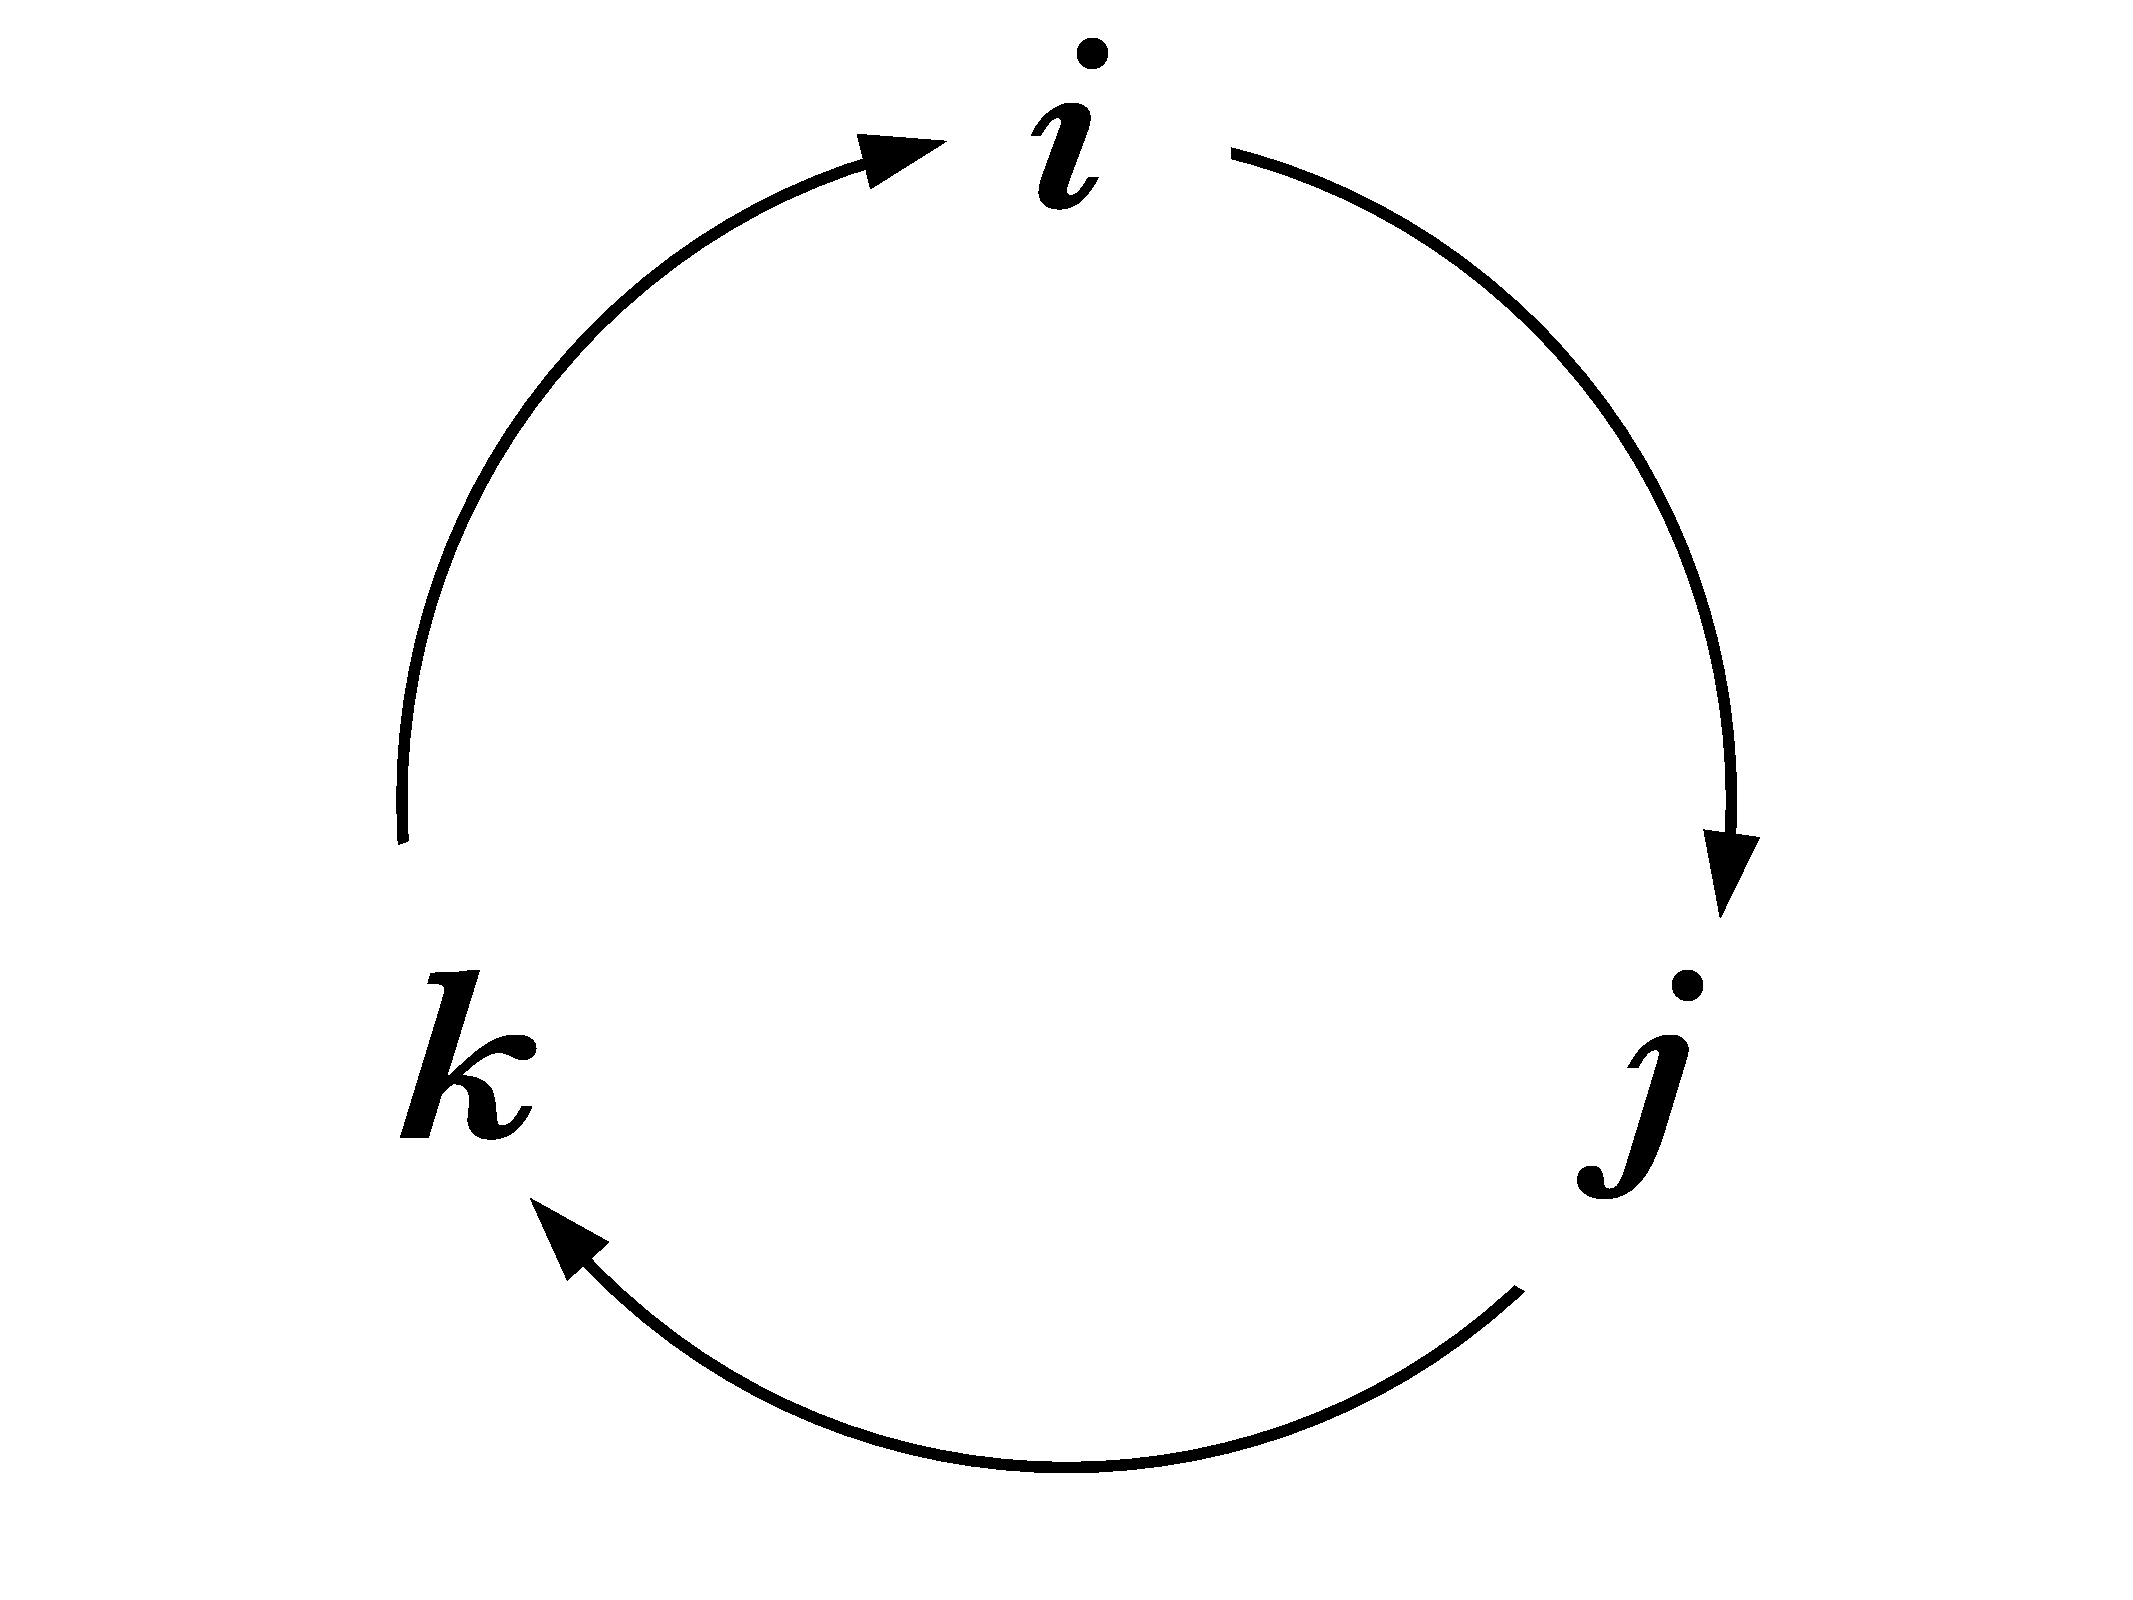
\includegraphics[width=0.3\linewidth]{Figures/quaternion_multiplication.pdf}
\caption{Diagrama ilustrando a regra de multiplica\c c\~ao entre as unidades imagin\'arias $ \qi $, $ \qj $ e $ \qk $.}
\label{fig:quatmult}
\end{figure}
\end{frame}

\begin{frame}{A \'algebra dos quat\'ernios}{Defini\c c\~oes e opera\c c\~oes}
\begin{itemize}
\item Parte \textbf{escalar} $ S(q) = a $ e \textbf{vetorial} $ \qV (q) = b\qi + c\qj + d\qk $.
\item Isomorfismo entre $ \qV (\mathbb{H}) $ e $ \mathbb{R}^3 $
\begin{itemize}
\item Produto vetorial
\item Produto escalar
\end{itemize}
\item O produto 
\begin{equation}
\small
\label{eq:q_prod}
\begin{aligned}
q_1 q_2 = &  \ (a_1 + b_1\qi + c_1\qj + d_1\qk) (a_2 +  b_2\qi + c_2\qj + d_2\qk)  \\ 
= & \ (a_1 a_2 - b_1 b_2 - c_1 c_2 - d_1 d_2)  \\
& + \qi (b_1 a_2 + a_1 b_2 - d_1 c_2 + c_1 d_2)  \\
& + \qj (c_1 a_2 + d_1 b_2 + a_1 c_2 - b_1 d_2)  \\
& + \qk (d_1 a_2 - c_1 b_2 + b_1 c_2 + a_1 d_2).
\end{aligned}
\end{equation}
pode ser reescrito como
\begin{equation}
\small
\label{eq:prod_vectors}
\begin{aligned}
q_1 q_2 = & \ S(q_1)S(q_2) - \langle\qV(q_1), \qV(q_2)\rangle \\
& + S(q_1) \qV(q_2) + S(q_2)\qV(q_1) + \qV(q_1) \times \qV(q_2).
\end{aligned}
\end{equation}
\end{itemize}
\end{frame}


\begin{frame}{A \'algebra dos quat\'ernios}{Defini\c c\~oes e opera\c c\~oes}
\begin{itemize}
\item Conjuga\c c\~ao: $ \bar{q} \overset{\Delta}{=} S(q) - V(q) $
\item Norma: $ |q| \overset{\Delta}{=} \sqrt{a^2 + b^2 + c^2 + d^2} $, $ |q|^2 = \bar{q} q = q \bar{q} $
\item Nomenclatura:
\begin{itemize}
\item Quat\'ernio unit\'ario: $ |q| = 1 $
\item Quat\'ernio puro: $ S(q) = 0 $
\item Quat\'ernios ortogonais: $ \qmu \perp \qnu \iff S(\qmu \qnu) = \langle \qmu, \qnu \rangle = 0$
\end{itemize}
\item Para dois quat\'ernios puros, unit\'arios e ortogonais $ \qmu $ e $ \qnu $, $ (\qmu, \qnu, \qmu \qnu) $ formam uma base ortonormal para $ \qV (\mathbb{H}) $.
\end{itemize}
\end{frame}

\begin{frame}{A \'algebra dos quat\'ernios}{Forma de Euler}
\begin{itemize}
\item Se $ \qmu $ \'e o quat\'ernio puro unit\'ario paralelo \`a parte vetorial de $ q $,
\begin{equation}
\label{eq:euler}
q = |q| e^{\qmu \theta} = |q|\cos \theta + |q|\qmu \sen \theta.
\end{equation}
\end{itemize}

\begin{block}{}
Todo quat\'ernio unit\'ario puro \'e uma raiz quadrada da unidade. Assim, $ \mathbb{C}_{\qmu} \overset{\Delta}{=} \{ a + \qmu b \ |\  a, b \in \mathbb{R} \}$ $ \mathbb{C}_{\qi} $ \'e isomorfo ao conjunto dos complexos.
\end{block}

\begin{itemize}
\item Seja o quat\'ernio unit\'ario puro $ \mathbf{\nu} $. De (\ref{eq:euler}),
\begin{equation}
%\label{key}
\mathbf{\nu} = |\mathbf{\nu}| e^{\mathbf{\nu} \theta}
\Rightarrow
\mathbf{\nu} = e^{\mathbf{\nu} \theta} \Rightarrow \theta = \pi
\end{equation}
portanto,
\begin{equation}
%\label{key}
\mathbf{\nu}^2 = \left( e^{\mathbf{\nu}\pi} \right)^2 = e^{\mathbf{\nu} 2\pi} = 1.
\end{equation}
\end{itemize}
\end{frame}

\begin{frame}{A \'algebra dos quat\'ernios}{Decomposi\c c\~ao simpl\'etica e similaridade}
\begin{itemize}
\item Uma vez que representamos por $ (\qmu, \qnu, \qmu \qnu) $ uma base gen\'erica para $ \qV(\mathbb{H}) $, todo quat\'ernio pode ser expresso em sua \textbf{decomposi\c c\~ao simpl\'etica}
\begin{equation}
\label{eq:decomposicao}
q = q^{(s)} + q^{(p)} \qnu, \quad q^{(s)}, q^{(p)} \in \mathbb{C}_{\qmu}.
\end{equation}

\item $ q, r \in \mathbb{H} $ s\~ao \textbf{similares} ($ q \sim r $) se e somente se $ \exists v \in \mathbb{H} $ n\~ao nulo tal que
\begin{equation}
v^{-1}q v = r.
\end{equation}
\begin{itemize}
\item Rota\c c\~ao no espa\c co 3D: dados $ v,x \in \mathbb{H} $, $ v = |v| e^{\qmu \alpha}$, a transforma\c c\~ao de similaridade
\begin{equation}
\label{eq:rotacao}
\phi_v(x) = v x v^{-1}
\end{equation}
produz a rota\c c\~ao da parte vetorial (imagin\'aria) de $ x $ em torno do eixo $ \qmu $ (que tem a mesma dire\c c\~ao da parte vetorial de $ v $) de um \^angulo $ 2\alpha $ \colorcite{\cite{ward2012quaternions}}, seguindo a regra da m\~ao direita.
\end{itemize}
\end{itemize}
\end{frame}

\begin{frame}{A transformada discreta de Fourier quaterni\^onica}{Ou \textit{quaternion discrete Fourier transform} (QDFT)}
\begin{itemize}
\item Se $ \qmu $ \'e um quat\'ernio unit\'ario puro qualquer, a $ m $-\'esima componente do vetor transformado pela QDFT unit\'aria de eixo $ \qmu $ \`a esquerda \'e dada por
\begin{equation}
\label{eq:QDFT_fwd}
\widehat{v}_m = \text{QDFT}\{ \mathbf{v} \}_m \overset{\Delta}{=} \frac{1}{\sqrt{N}} \sum_{n=0}^{N-1}  \exp \left( -\qmu \frac{2\pi}{N} nm \right) v_n \in \mathbb{C}_{\qmu},
\end{equation}
com a f\'ormula da transforma\c c\~ao inversa trazendo a m\'ultiplica\c c\~ao pelo n\'ucleo tamb\'em \`a esquerda:
\begin{equation}
\label{eq:QDFT_inv}
v_n = \text{QDFT}^{-1}\{ \widehat{\mathbf{v}} \}_n = \frac{1}{\sqrt{N}}\sum_{m=0}^{N-1}  \exp \left( \qmu \frac{2\pi}{N} nm \right) \widehat{v}_m.
\end{equation}
\end{itemize}
\end{frame}

\begin{frame}{A transformada discreta de Fourier quaterni\^onica}{Representa\c c\~ao matricial}
\begin{itemize}
\item As equa\c c\~oes de an\'alise e s\'intese podem ser escritas em forma matricial como
\begin{equation}
\label{eq:QDFT}
\widehat{\mathbf{v}} = \text{QDFT}\{ \mathbf{v} \} = \mathbf{F} \mathbf{v},
\end{equation}
\begin{equation}
\label{eq:QDFT_mtx_inv}
\mathbf{v} = \text{QDFT}^{-1}\{ \widehat{\mathbf{v}} \} = \mathbf{F}^{-1} \widehat{\mathbf{v}},
\end{equation}
em que $ \mathbf{F} $ \'e a matriz da transformada unit\'aria,
%--multiplicando sempre \`a esquerda--,
com entradas $ \{\mathbf{F}\}_{n,m} = \sqrt{N}^{-1} \exp \left( -\qmu \frac{2\pi}{N} nm \right)$.
\item Uso da decomposi\c c\~ao simpl\'etica no c\'alculo da QDFT,
\begin{equation}
\small
\begin{aligned}
%\label{eq:QDFT_fwd}
\text{QDFT}\{ \mathbf{x} \}_m &= \frac{1}{\sqrt{N}} \sum_{n=0}^{N-1} \exp \left( -\qmu \frac{2\pi}{N} nm \right) x_n \\
&= \frac{1}{\sqrt{N}} \sum_{n=0}^{N-1} \exp \left( -\qmu \frac{2\pi}{N} nm \right) (x_n^{(s)} + x_n^{(p)}\qnu) \\
&= \text{DFT}_{\qmu}\{ \mathbf{x}^{(s)} \}_m +
\text{DFT}_{\qmu}\{ \mathbf{x}^{(p)} \}_m \qnu,
\end{aligned}
\end{equation}
\end{itemize}
\end{frame}

\begin{frame}{Princ\'ipios do processamento de sinais sobre grafos}
\begin{itemize}
\item Em diversos contextos, os sinais de interesse est\~ao naturalmente definidos sobre uma estrutura em rede, modelada como um grafo \colorcite{\cite{alam2015toward,nguyen2014compression,goldsberry2017brain,leonardi2013tight}}.

\vspace{-0.1\textheight}
\begin{figure}
\centering
\subfloat[\label{figa_graphs}]{
	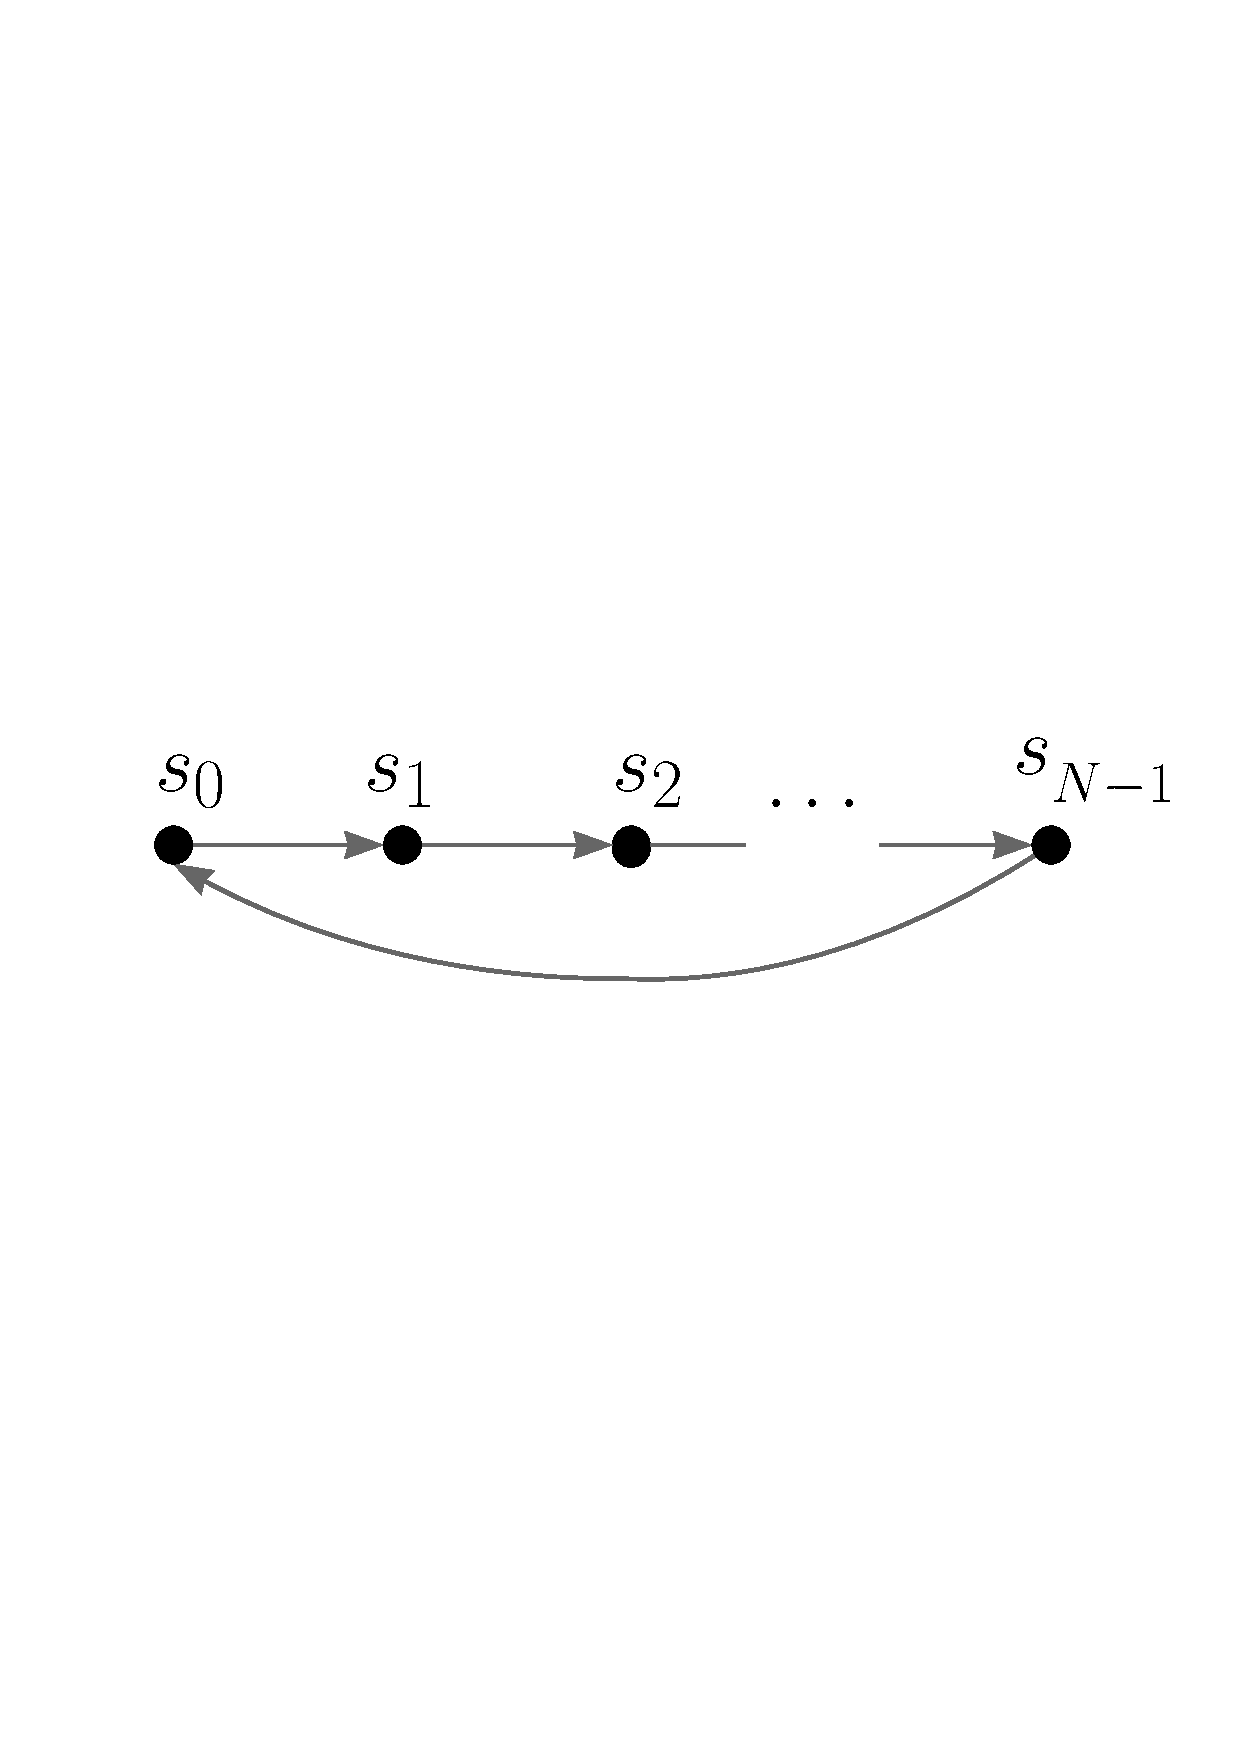
\includegraphics[width=0.3\linewidth]{Figures/signal_ring_graph_white_border.pdf}
}
\subfloat[\label{figb_graphs}]{
	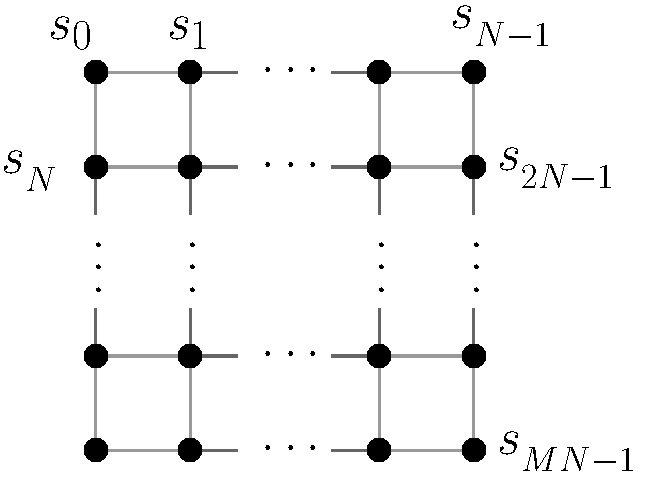
\includegraphics[width=0.3\linewidth]{Figures/image_graph.pdf}
}%
\subfloat[\label{figd_graphs}]{
	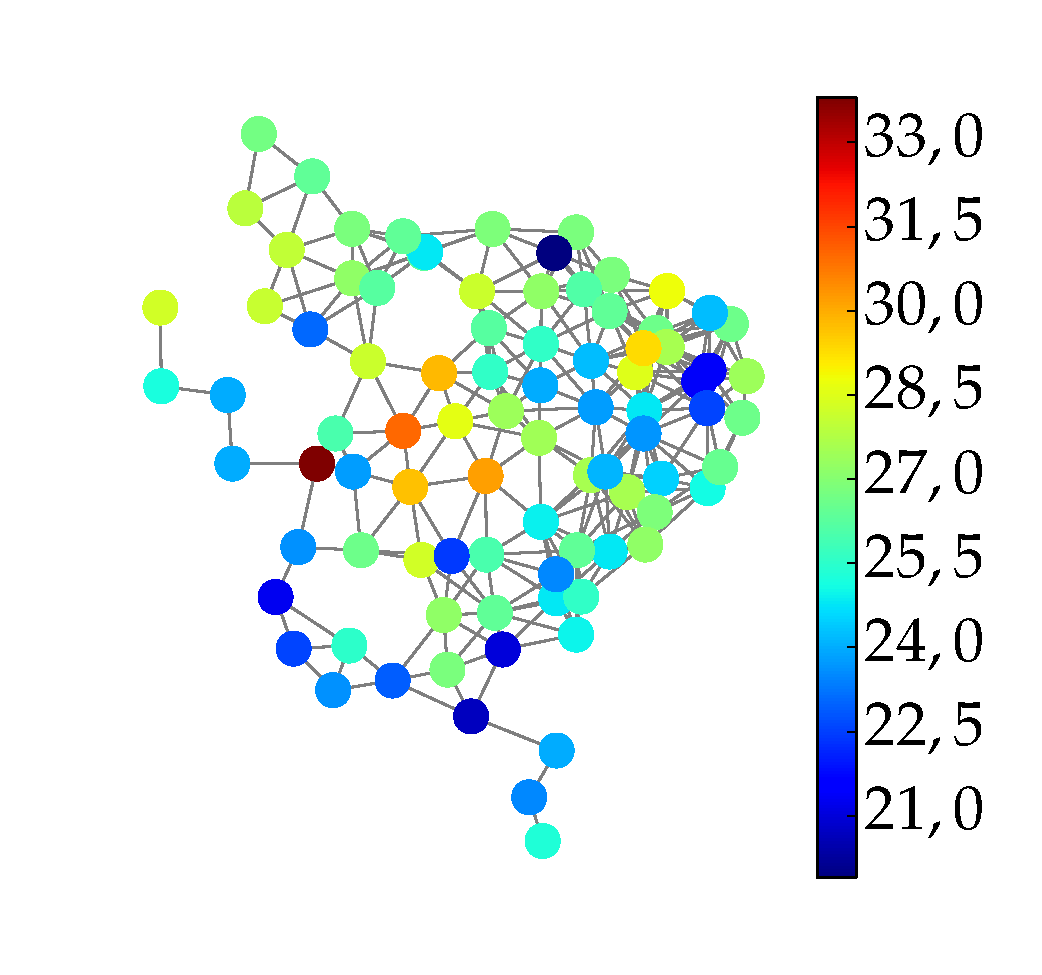
\includegraphics[width=0.32\linewidth]{Figures/temp_NE_stretched.pdf} }%
\caption{Representa\c{c}\~oes de sinais sobre (a) um grafo em anel direcionado, (b) um grafo em grade retangular uniforme  e (c) um grafo formado por cidades do Nordeste brasileiro.}%
\label{fig:graphs}%
%	\vspace{-0.9cm}
%	{\\ \small Fonte: o autor.}
\end{figure}
\end{itemize}
\end{frame}

\begin{frame}{Princ\'ipios do processamento de sinais sobre grafos}{Defini\c c\~oes}
\begin{itemize}
\item Um sinal $ \mathbf{s} $ sobre um grafo $ \mathcal{G} = \{\mathcal{V}, \mathbf{A}\} $, com $ |\mathcal{V}| = N $, \'e definido como
\begin{equation}
%\label{key}
s: \ \mathcal{V} \rightarrow \mathbb{C} \ | \ s(v_i) = s_i,
\end{equation}
i.~e. \'e um vetor em $ \mathbb{C}^N $ \emph{indexado pelos v\'ertices de} $ \mathcal{G} $.
\item A matriz de adjac\^encia $ \mathbf{A} $ traz em sua entrada $ A_{ij} $ o peso da aresta indo de $ v_j $ para $ v_i $
\begin{itemize}
\item \'E uma das principais op\c c\~oes de \textbf{operador de deslocamento} de sinal sobre grafo.
\end{itemize}
\end{itemize}

%\vspace{-0.01\textheight}
\begin{figure}
\centering
\includegraphics[width=0.7\linewidth]{Figures/unit_shift_keynote}
\caption{Exemplo de deslocamento unit\'ario.}
\end{figure}
\end{frame}

\begin{frame}{Princ\'ipios do processamento de sinais sobre grafos}{Autofun\c c\~oes do deslocamento unit\'ario e a GFT}
\begin{itemize}
\item Grafo em anel $ \rightarrow $ modelo do tempo discreto. Matriz de adjac\^encia:
\begin{equation}\label{eq:C}
\mathbf{C} =
\left[\renewcommand{\arraystretch}{0.65}\begin{array}{cccc}
&  &  &   1\\ 
1 &  &   & \\ 
&   \ddots &  & \\ 
&  &   1 & 
\end{array}\right],
\end{equation}
\item \textit{Transformada de Fourier de tempo discreto} (TFTD): decomposi\c c\~ao na base de autofun\c c\~oes da filtragem LIT
\end{itemize}
\end{frame}


\section{Fracionariza\c c\~ao da QDFT}\label{sec:cnt}

\begin{frame}{A autoestrutura da QDFT}
Como visto em (\ref{eq:QDFT_fwd}), a equa\c c\~ao se an\'alise da QDFT \'e
\begin{equation}
%\label{eq:QDFT_fwd}
\widehat{v}_m = \text{QDFT}\{ \mathbf{v} \}_m \overset{\Delta}{=} \frac{1}{\sqrt{N}} \sum_{n=0}^{N-1}  \exp \left( -\qmu \frac{2\pi}{N} nm \right) v_n \in \mathbb{C}_{\qmu},
\end{equation}
ou, em forma matricial,
\begin{equation}
\widehat{\mathbf{v}} = \text{QDFT}\{ \mathbf{v} \} = \mathbf{F} \mathbf{v},
\end{equation}
com $ \{\mathbf{F}\}_{n,m} = \sqrt{N}^{-1} \exp \left( -\qmu \frac{2\pi}{N} nm \right)$.
\end{frame}

\begin{frame}{foo}
\begin{teorema}
\label{th:01}
Seja $ \mathbf{v} $ um autovetor da DFT unit\'aria com autovalor $ \lambda $.
\begin{itemize}
\item[(a)] Se $ \mathbf{v} $ tem simetria par (caso em que $ \lambda = \pm 1 $), ent\~ao ele tamb\'em \'e um autovetor da QDFT com autovalor $ \lambda $.
\item[(b)] Se $ \mathbf{v} $ tem simetria \'impar (caso em que $ \lambda = \pm \qi $), ent\~ao ele \'e um autovetor da QDFT de eixo $ \qmu $ com autovalor $ -\lambda \qi \qmu$, i.~e. $ \pm \qmu $.
%Se $ \qmu = \qj $, ent\~ao seu autovalor \'e $ -\lambda \qk $.
\end{itemize}
\end{teorema}
\end{frame}

\begin{frame}{foo}
\begin{center}
\captionof{table}{Autovalores da DFT e da QDFT.}
\label{tab:01}
\begin{tabular}{ccc}
\toprule
\shortstack{Simetria do\\autovetor} & \shortstack{Autovalor\\(DFT)} & \shortstack{Autovalor\\(QDFT)} \\
\midrule
Par & $ \pm 1 $ & $ \pm 1 $ \\
\'Impar & $ \pm \qi $ & $ - (\pm \qi) \qi \qmu = \pm \qmu $\\
\bottomrule
\end{tabular}
\end{center}
\end{frame}

\begin{frame}{2D-QDFT e imagens coloridas com camada de opacidade}
\begin{figure}
\centering
\subfloat[\label{fig:dice}]{
	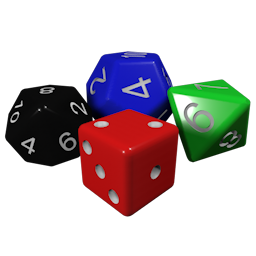
\includegraphics[width=0.25\linewidth]{Figures/dice_256x256.png}
}~
\subfloat[]{
	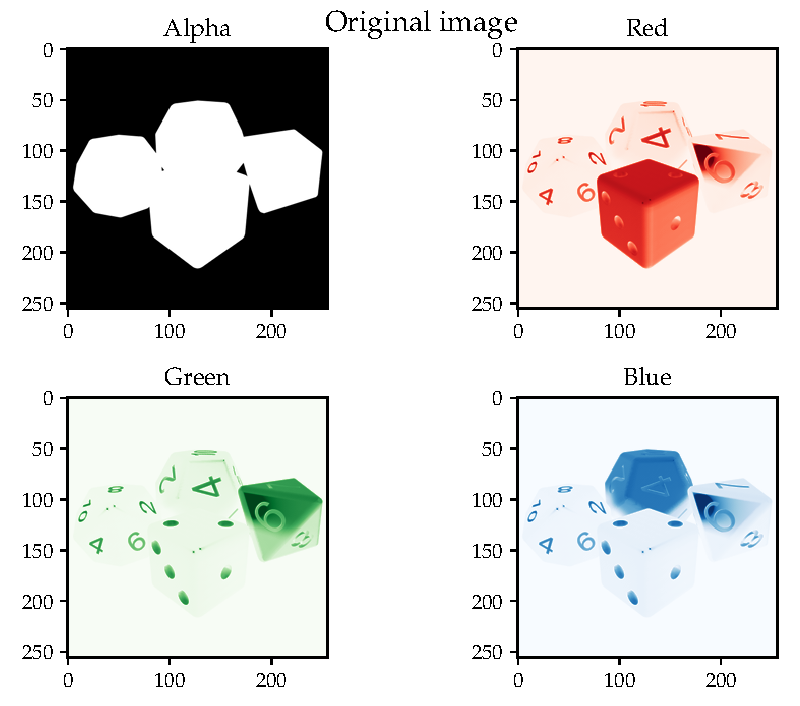
\includegraphics[width=0.35\linewidth]{Figures/dice_256x256_layers.pdf}
}~
\subfloat[]{
	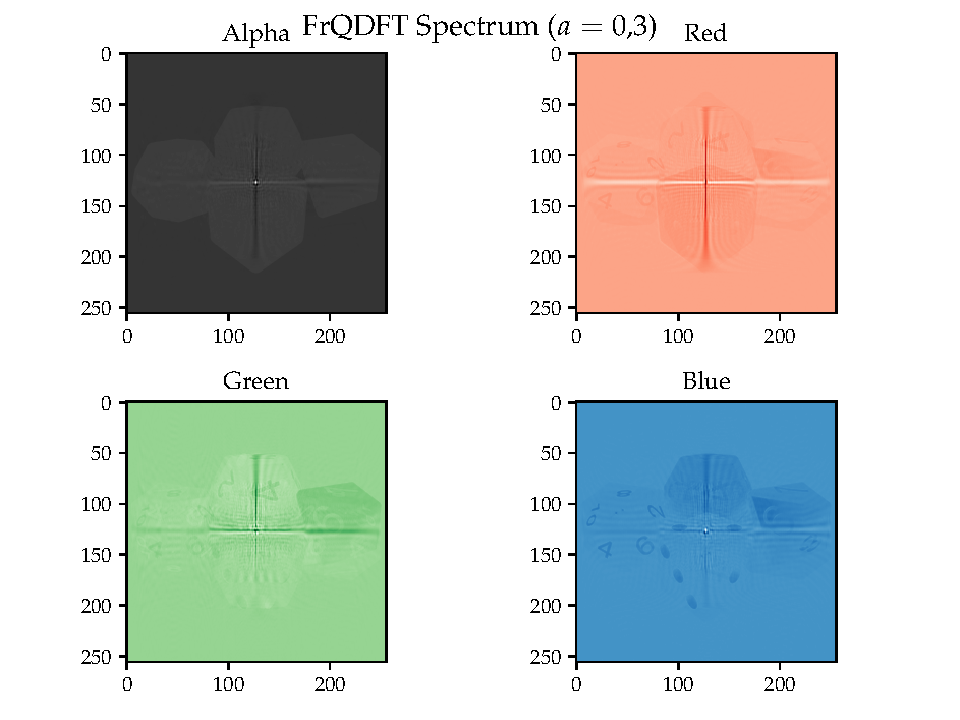
\includegraphics[width=0.35\linewidth]{Figures/dice_256x256_layers_frqdft.pdf}
}~
\caption{(a) Imagem de teste em formato PNG. (b) Visualiza\c c\~ao de cada uma das quatro camadas da imagem e (c) de seu espectro pela FrQDFT com $ \qmu = \frac{1}{\sqrt{3}}(\qi + \qj + \qk) $ e $ a=0{,}3 $.}
\end{figure}
\end{frame}

\begin{frame}{2D-QDFT e imagens coloridas com camada de opacidade}
\begin{figure}
	\centering
	\subfloat[\label{fig:2D_QDFTv1}]{
		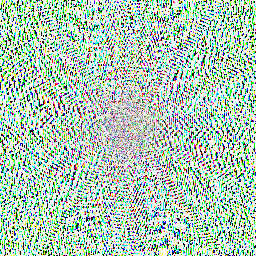
\includegraphics[width=0.35\linewidth]{Figures/2D_QDFTv1.png}
	}~
	\subfloat[\label{fig:2D_QDFTv2}]{
		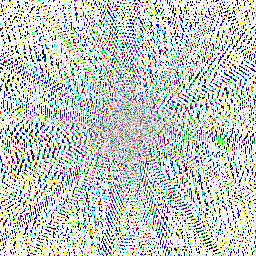
\includegraphics[width=0.35\linewidth]{Figures/2D_QDFTv2.png}
	}
	\caption{(a) 2D-QDFT da imagem na Fig. \ref{fig:dice} segundo (\ref{eq:2DQDFT}), com eixo $ \qmu = \frac{1}{\sqrt{3}}(\qi + \qj + \qk) $. (b) 2D-QDFT da mesma imagem, com mesmo eixo, segundo defini\c c\~ao alternativa em (\ref{eq:2DQDFTv2}).}
	\label{fig:QDFT}
\end{figure}
\end{frame}

\begin{frame}{Esquema de cifragem via MFrQDFT}
\begin{figure}
	\centering
	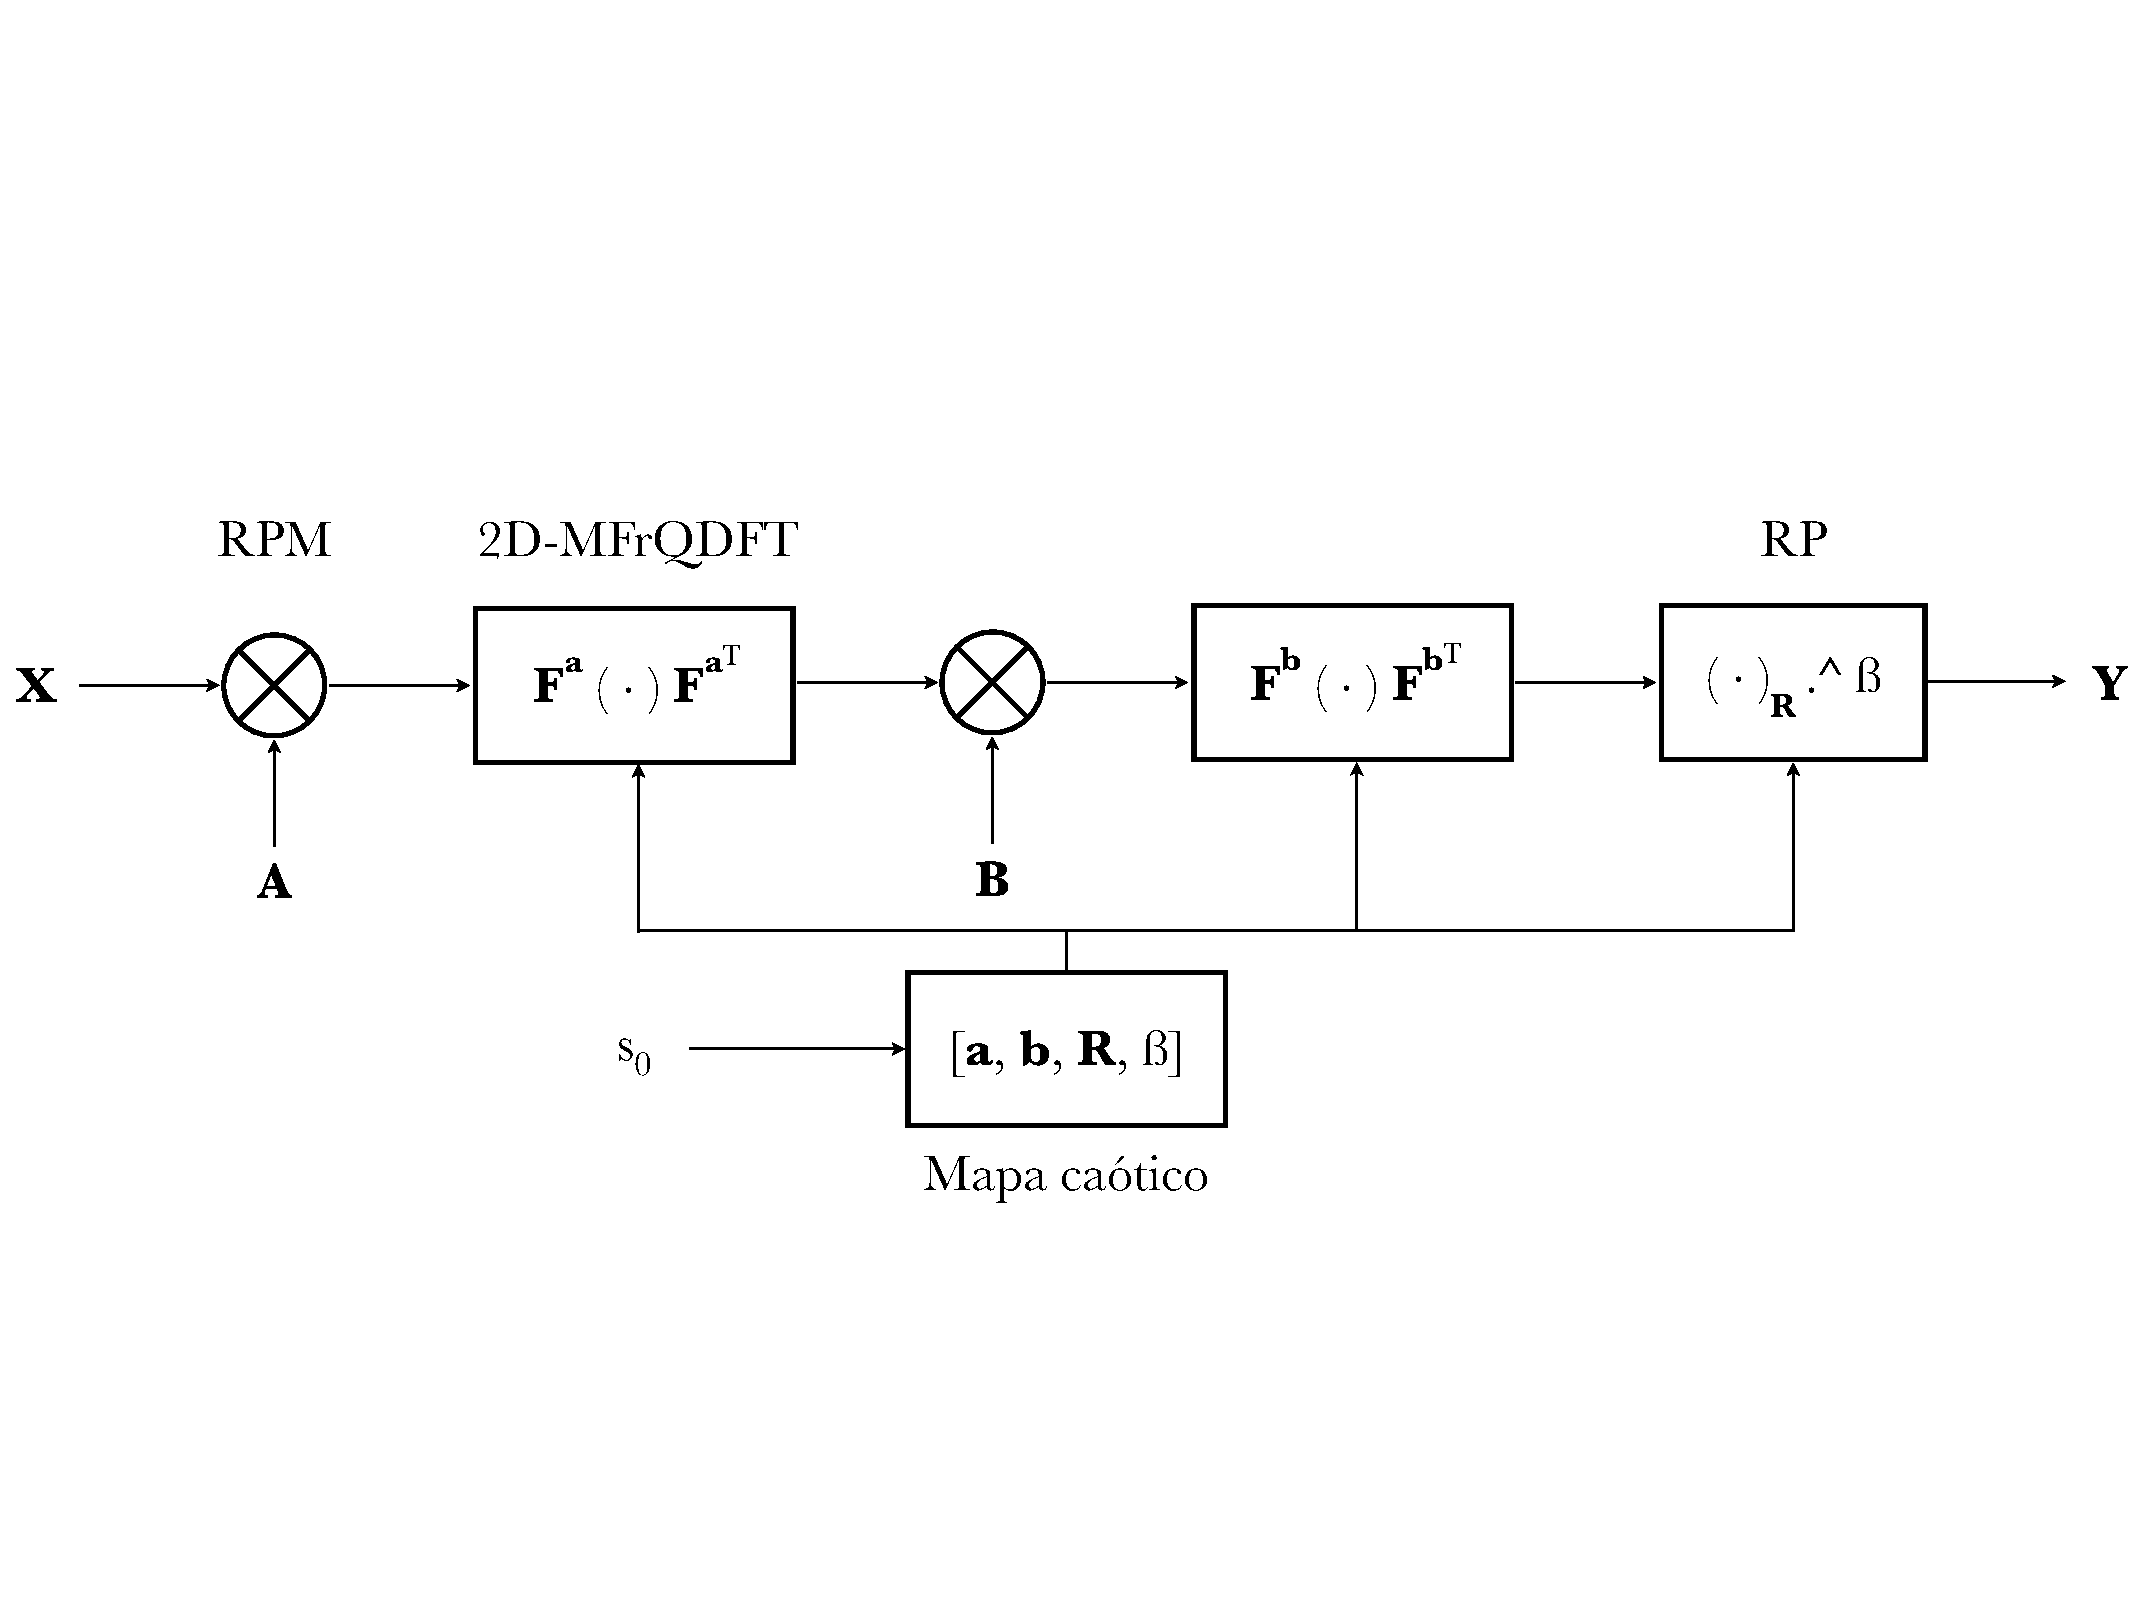
\includegraphics[width=0.99\linewidth]{Figures/esquema_PT.pdf}
	\caption{Esquema de cifragem proposto, explorando a MFrQDFT.}
	\label{fig:cifragem}
\end{figure}
\end{frame}
 
\begin{frame}{Esquema de cifragem via MFrQDFT}{Exemplo}
\begin{figure}
\centering
\subfloat[\label{fig:ciphered01}]{
	
\includegraphics[width=0.3\linewidth]{Figures/sage_Encrypted_image.png}
}~
\subfloat[\label{fig:ciphered02}]{
	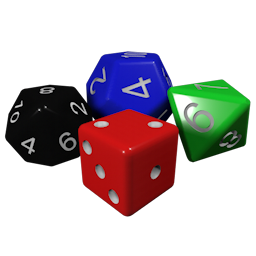
\includegraphics[width=0.35\linewidth]{Figures/Decrypted_image_error_0.png}
}~
\subfloat[\label{fig:ciphered03}]{
	
\includegraphics[width=0.3\linewidth]{Figures/sage_Decrypted_image_error_minus1dot6.png}
}~
\caption{(a) Imagem cifrada. (b) Imagem decifrada com a chave $ s_0 $ correta. (c) Imagem decifrada com a chave errada $ \widetilde{s_0} = s_0 + \epsilon $, com $ \epsilon = -1{,}6 \cdot 10^{-80} $.}
\end{figure}
\end{frame}


\begin{frame}{Esquema de cifragem via MFrQDFT}{Efeito de erro na chave na reconstru\c c\~ao da imagem}
\begin{figure}
\centering
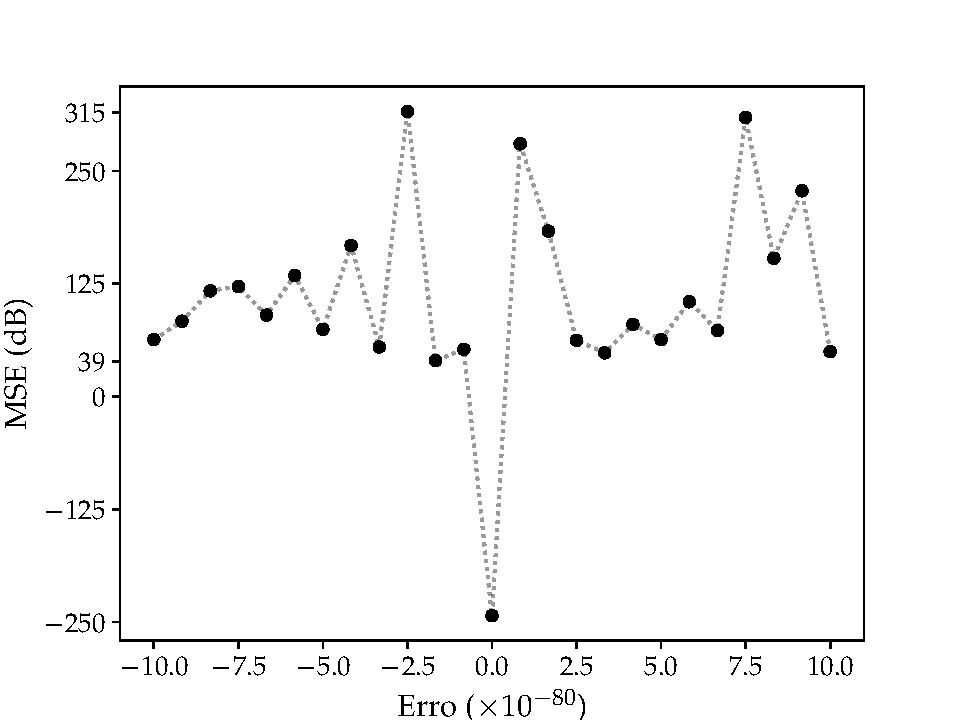
\includegraphics[width=0.7\linewidth]{Figures/MSEdb_FrQDFT_PT.pdf}
\caption{Erro m\'edio quadr\'atico, em dB, da imagem decifrada, em fun\c c\~ao do erro $ \epsilon $ imposto \`a chave.}
\label{fig:MSE}
\end{figure}
\end{frame}

\section[QGSP]{Em busca de QGSP}\label{sec:gfnt}

%\begin{frame}{GFNT: computational experiments}
%\begin{figure}
%\centering
%\subfloat[\label{fig:graphsgfnt01}]{
%\includegraphics[height=0.6\textheight]{Figures/sample01.png}
%}~
%\subfloat[\label{fig:graphsgfnt02}]{
%\includegraphics[height=0.6\textheight]{Figures/sample02.png}
%}
%\caption{(a) An arbitrary graph ($N=6$) and (b) a random interval graph ($N=16$). The numbers inside the circles indicate the vertex indexes.}
%\label{fig:graphsgfnt}
%\end{figure}
%\end{frame}

\section{Considera\c c\~oes finais}\label{sec:conc}

\begin{frame}{Publica\c c\~oes}
\begin{itemize}
\item Ribeiro, G. B., e Lima, J. B. ``Eigenstructure and fractionalization of the quaternion discrete Fourier transform.'' \emph{Optik} (2019): 163957. DOI: \colorlink{\href{https://doi.org/10.1016/j.ijleo.2019.163957}{10.1016/j.ijleo.2019.163957}}.

\item Ribeiro, G. B., e Lima, J. B. ``The Cosine Number Transform: A Graph Signal Processing Approach''. 2019 IEEE Global Conference on Signal and Information Processing (GlobalSIP) (pp. 1-5). IEEE. DOI: \colorlink{\href{https://doi.org/10.1109/GlobalSIP45357.2019.8969165}{10.1109/GlobalSIP45357.2019.8969165}}.
\end{itemize}
\end{frame}

% Bibliography
%\input{mybib}
%\bibliography{mybib} 
%\bibliographystyle{ieeetr}
% All of the following is optional and typically not needed. 
%\appendix
\section<presentation>*{\appendixname}
\subsection<presentation>*{References}

\begin{frame}[allowframebreaks]
  \frametitle<presentation>{References}
  \addtocounter{framenumber}{-1}
%  \nocite{*}
  \bibliographystyle{apalike}
  \bibliography{mybib}
  
\vfill
%\begin{center}
%\small
%Contato: \\
%\href{mailto:guilherme.boaviagem@gmail.com}{\emph{guilherme.boaviagem@gmail.com}}
%\end{center}
\end{frame}
% ---------------------
\end{document}